\section{Configuration Data}

We applied our framework to Cisco configurations of core, border, and distribution routers from three large university networks(Table~\ref{tab:datasets}). The figure below shows us the distribution by size for configurations from all universities combined. Additionally, we were also able to get extensive data from University A's version control histories. This allowed us to perform some tests based on snapshots sampled across time. We used monthly time intervals for such tests.

\begin{table}
    \small \centering
    \begin{tabular}{ | c | c | c | c |}
    \hline
        {\bf Univ.} & {\bf No. of Configs} & {\bf Total Lines} & {\bf Avg
    Lines} \\ 
    \hline
    A & 35 & 73K & 2.1K \\ 
    B & 26 & 61K & 2.3K \\ 
    C & 24 & 67K & 2.8K \\ 
    \hline
    \end{tabular}
    \caption{Configurations used in our evaluation}
    \vspace{-1em}
    \label{tab:datasets}
\end{table}

\begin{figure}[H]
	\centering
	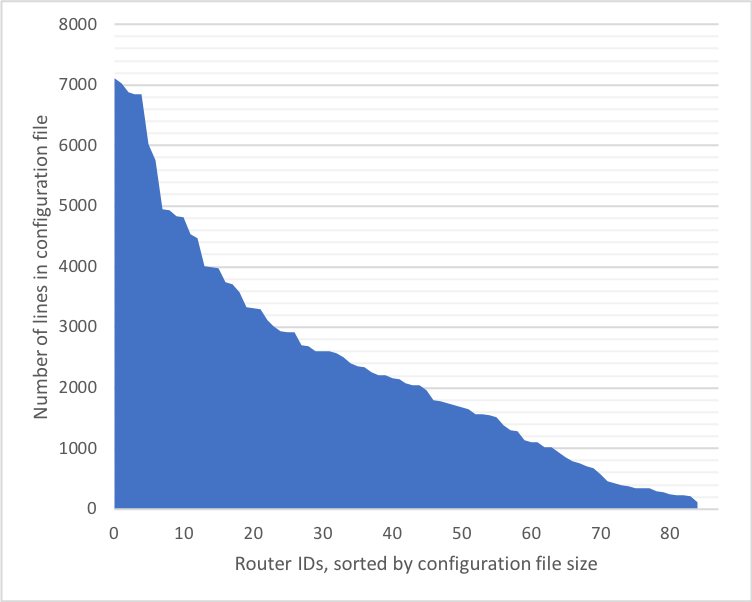
\includegraphics[width=5in]{config_sizes.png}
	\caption{Our data has a good mixture of long and short configurations}
\end{figure}
